% LinearSpan_GC_doc.tex
% LuaLaTeX document explaining the mathematical content of LinearSpan_GC.lean
% Compile with: lualatex LinearSpan_GC_doc.tex

\documentclass[a4paper,11pt]{ltjsarticle}

% ===== パッケージ =====
\usepackage{luatexja}
\usepackage{luatexja-fontspec}
\usepackage{amsmath, amssymb, amsthm}
\usepackage{mathtools}
\usepackage{tikz}
\usepackage{tikz-cd}
\usetikzlibrary{arrows.meta, positioning, shapes.geometric}
\usepackage{hyperref}
\usepackage{cleveref}
\usepackage{tcolorbox}
\tcbuselibrary{theorems, skins, breakable}
\usepackage{listings}
\usepackage{xcolor}

% ===== フォント設定 =====
% システムにNoto Sans CJK JPがない場合はコメントアウトしてください
% \setmainjfont{Noto Sans CJK JP}
% \setsansjfont{Noto Sans CJK JP}

% ===== 定理環境 =====
\theoremstyle{definition}
\newtheorem{definition}{定義}[section]
\newtheorem{theorem}[definition]{定理}
\newtheorem{lemma}[definition]{補題}
\newtheorem{proposition}[definition]{命題}
\newtheorem{corollary}[definition]{系}
\newtheorem{example}[definition]{例}
\newtheorem{remark}[definition]{注意}

% ===== Leanコード用設定 =====
\definecolor{leanblue}{RGB}{0, 0, 180}
\definecolor{leangreen}{RGB}{0, 128, 0}
\definecolor{leangray}{RGB}{128, 128, 128}

\lstdefinelanguage{Lean4}{
  keywords={def, theorem, lemma, example, abbrev, noncomputable, where, by, intro, exact, simp, rfl, fun, show},
  keywordstyle=\color{leanblue}\bfseries,
  ndkeywords={StructureTowerWithMin, GaloisConnection, ClosureOperator, Set, Submodule, Vec2Q},
  ndkeywordstyle=\color{leangreen},
  commentstyle=\color{leangray}\itshape,
  morecomment=[l]{--},
  morecomment=[s]{/-}{-/},
  stringstyle=\color{red},
  basicstyle=\ttfamily\small,
  breaklines=true,
  frame=single,
  backgroundcolor=\color{gray!10},
}

\lstset{language=Lean4}

% ===== カスタムボックス =====
\newtcolorbox{keyinsight}{
  colback=blue!5!white,
  colframe=blue!75!black,
  fonttitle=\bfseries,
  title=核心的洞察,
  breakable
}

\newtcolorbox{leancode}{
  colback=gray!5!white,
  colframe=gray!75!black,
  fonttitle=\bfseries,
  title=Lean 4 形式化,
  breakable
}

% ===== タイトル =====
\title{%
  \textbf{線形包とGalois接続}\\[0.5em]
  \Large 構造塔理論への橋渡し
}

\author{%
  \textbf{TeX文書生成}: Claude (Anthropic)\\
  \textbf{Lean形式化}: Antigravity (Google DeepMind)\\[0.5em]
  \small 2025年12月26日
}

\date{}

% ===== 本文 =====
\begin{document}

\maketitle

\begin{abstract}
本文書は、線形代数における\textbf{線形包}（linear span）が\textbf{Galois接続}を形成すること、
および\textbf{構造塔}（StructureTowerWithMin）の具体例として$\mathbb{Q}^2$上の基底カウント階層を
形式化した内容を数学的に解説する。
これらの形式化は Lean 4 + Mathlib で実装され、
抽象的な圏論的構造と具体的な線形代数の間の橋渡しを提供する。
\end{abstract}

\tableofcontents

\newpage

%%%%%%%%%%%%%%%%%%%%%%%%%%%%%%%%%%%%%%%%%%%%%%%%%%%%%%%%%%%%%%%%%%%%%%%%%%%%%%%
\section{序論：Galois接続と閉包作用素}
%%%%%%%%%%%%%%%%%%%%%%%%%%%%%%%%%%%%%%%%%%%%%%%%%%%%%%%%%%%%%%%%%%%%%%%%%%%%%%%

\subsection{Galois接続の基本}

\begin{definition}[Galois接続]
  二つの半順序集合 $(P, \leq_P)$ と $(Q, \leq_Q)$ の間の\textbf{Galois接続}（Galois connection）とは、
  関数の対 $(\ell, u)$ であって
  \[
    \ell : P \to Q, \quad u : Q \to P
  \]
  が次の随伴条件を満たすものである：
  \[
    \forall p \in P,\, \forall q \in Q:\quad \ell(p) \leq_Q q \iff p \leq_P u(q)
  \]
  このとき $\ell$ を\textbf{下随伴}（lower adjoint）、$u$ を\textbf{上随伴}（upper adjoint）と呼び、
  $\ell \dashv u$ と書く。
\end{definition}

\begin{figure}[htbp]
  \centering
  \begin{tikzcd}[row sep=large, column sep=huge]
    P \arrow[r, bend left=25, "\ell"{name=F}] 
    & Q \arrow[l, bend left=25, "u"{name=G}]
    \arrow[phantom, from=F, to=G, "\dashv" rotate=-90]
  \end{tikzcd}
  \caption{Galois接続 $\ell \dashv u$ の図式}
  \label{fig:galois-connection}
\end{figure}

\subsection{閉包作用素との関係}

Galois接続から自然に閉包作用素が導出される。

\begin{definition}[閉包作用素]
  半順序集合 $(P, \leq)$ 上の\textbf{閉包作用素}（closure operator）とは、
  関数 $c : P \to P$ であって以下の三条件を満たすものである：
  \begin{enumerate}
    \item \textbf{拡大性}（extensive）：$\forall x \in P,\, x \leq c(x)$
    \item \textbf{単調性}（monotone）：$x \leq y \Rightarrow c(x) \leq c(y)$
    \item \textbf{冪等性}（idempotent）：$c(c(x)) = c(x)$
  \end{enumerate}
\end{definition}

\begin{proposition}
  Galois接続 $\ell \dashv u$ が与えられたとき、合成 $c := u \circ \ell : P \to P$ は
  閉包作用素である。
\end{proposition}

\begin{figure}[htbp]
  \centering
  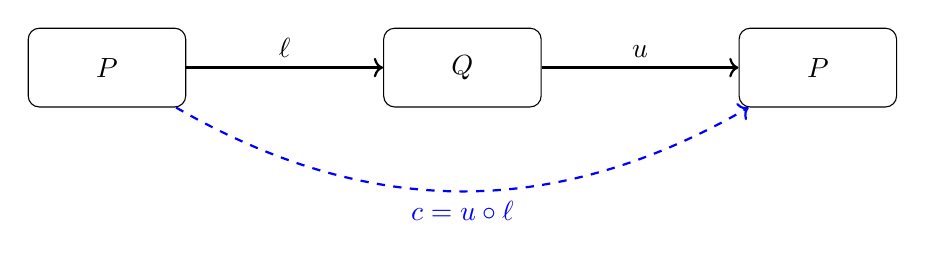
\begin{tikzpicture}[
    node distance=2.5cm,
    box/.style={draw, rounded corners, minimum width=2cm, minimum height=1cm}
  ]
    \node[box] (P1) {$P$};
    \node[box, right=of P1] (Q) {$Q$};
    \node[box, right=of Q] (P2) {$P$};
    
    \draw[->, thick] (P1) -- node[above] {$\ell$} (Q);
    \draw[->, thick] (Q) -- node[above] {$u$} (P2);
    \draw[->, thick, blue, dashed] (P1) to[bend right=30] node[below] {$c = u \circ \ell$} (P2);
  \end{tikzpicture}
  \caption{Galois接続から導出される閉包作用素}
  \label{fig:closure-from-gc}
\end{figure}

%%%%%%%%%%%%%%%%%%%%%%%%%%%%%%%%%%%%%%%%%%%%%%%%%%%%%%%%%%%%%%%%%%%%%%%%%%%%%%%
\section{DoD-1：線形包はGalois接続を形成する}
%%%%%%%%%%%%%%%%%%%%%%%%%%%%%%%%%%%%%%%%%%%%%%%%%%%%%%%%%%%%%%%%%%%%%%%%%%%%%%%

\subsection{核心的観察}

体 $K$ 上のベクトル空間 $V$ において、\textbf{線形包}（linear span）と\textbf{部分空間への包含}
の間には自然なGalois接続が存在する。

\begin{keyinsight}
  線形包の基本性質
  \[
    \operatorname{span}_K(S) \leq P \iff S \subseteq P
  \]
  はまさにGalois接続の随伴条件そのものである。
\end{keyinsight}

\subsection{形式的定義}

\begin{theorem}[線形包のGalois接続]
  体 $K$ 上のベクトル空間 $V$ に対して、以下の対がGalois接続を形成する：
  \begin{align*}
    \ell &: \mathcal{P}(V) \to \operatorname{Sub}_K(V), \quad S \mapsto \operatorname{span}_K(S) \\
    u &: \operatorname{Sub}_K(V) \to \mathcal{P}(V), \quad P \mapsto P \text{（underlying set）}
  \end{align*}
  ここで $\mathcal{P}(V)$ は $V$ の冪集合（包含順序）、$\operatorname{Sub}_K(V)$ は $V$ の部分$K$-加群全体（包含順序）である。
\end{theorem}

\begin{figure}[htbp]
  \centering
  \begin{tikzcd}[row sep=large, column sep=huge]
    \mathcal{P}(V) \arrow[r, bend left=25, "\operatorname{span}_K"{name=F}] 
    & \operatorname{Sub}_K(V) \arrow[l, bend left=25, "\text{coe}"{name=G}]
    \arrow[phantom, from=F, to=G, "\dashv" rotate=-90]
  \end{tikzcd}
  \caption{線形包のGalois接続}
  \label{fig:span-gc}
\end{figure}

\subsection{閉包作用素としての線形包}

\begin{corollary}
  合成 $c := \operatorname{coe} \circ \operatorname{span}_K : \mathcal{P}(V) \to \mathcal{P}(V)$ は
  閉包作用素である。すなわち、任意の $S \subseteq V$ に対して：
  \begin{enumerate}
    \item $S \subseteq \operatorname{span}_K(S)$（拡大性）
    \item $S \subseteq T \Rightarrow \operatorname{span}_K(S) \subseteq \operatorname{span}_K(T)$（単調性）
    \item $\operatorname{span}_K(\operatorname{span}_K(S)) = \operatorname{span}_K(S)$（冪等性）
  \end{enumerate}
\end{corollary}

\begin{leancode}
\begin{lstlisting}
theorem span_gc :
    GaloisConnection (fun s : Set V => Submodule.span K s)
                     (fun P : Submodule K V => (P : Set V)) := by
  intro s P
  exact Submodule.span_le

noncomputable def spanClosureOp : ClosureOperator (Set V) where
  toFun := fun s => (Submodule.span K s : Set V)
  monotone' := by intro s t h; exact Submodule.span_mono h
  le_closure' := by intro s x hx; exact Submodule.subset_span hx
  idempotent' := by intro s; ext x; constructor <;> ...
\end{lstlisting}
\end{leancode}

%%%%%%%%%%%%%%%%%%%%%%%%%%%%%%%%%%%%%%%%%%%%%%%%%%%%%%%%%%%%%%%%%%%%%%%%%%%%%%%
\section{DoD-2：構造塔としての基底カウント階層}
%%%%%%%%%%%%%%%%%%%%%%%%%%%%%%%%%%%%%%%%%%%%%%%%%%%%%%%%%%%%%%%%%%%%%%%%%%%%%%%

\subsection{構造塔の定義}

\begin{definition}[StructureTowerWithMin]
  \textbf{構造塔}（Structure Tower with Minimum）は以下のデータからなる：
  \begin{itemize}
    \item \textbf{基礎集合} $X$（carrier）
    \item \textbf{添字集合} $I$（Index）：前順序付き
    \item \textbf{層関数} $\operatorname{layer} : I \to \mathcal{P}(X)$
    \item \textbf{最小層関数} $\operatorname{minLayer} : X \to I$
  \end{itemize}
  これらは以下の公理を満たす：
  \begin{enumerate}
    \item \textbf{被覆性}：$\forall x \in X,\, \exists i \in I,\, x \in \operatorname{layer}(i)$
    \item \textbf{単調性}：$i \leq j \Rightarrow \operatorname{layer}(i) \subseteq \operatorname{layer}(j)$
    \item \textbf{最小層の所属}：$x \in \operatorname{layer}(\operatorname{minLayer}(x))$
    \item \textbf{最小性}：$x \in \operatorname{layer}(i) \Rightarrow \operatorname{minLayer}(x) \leq i$
  \end{enumerate}
\end{definition}

\subsection{具体例：$\mathbb{Q}^2$ の基底カウント}

$\mathbb{Q}^2$ 上で、標準基底 $\{e_1, e_2\}$ に関する「必要な基底ベクトル数」による階層を考える。

\begin{definition}[minBasisCount]
  ベクトル $v = (a, b) \in \mathbb{Q}^2$ に対して：
  \[
    \operatorname{minBasisCount}(v) := 
    \begin{cases}
      0 & \text{if } v = (0, 0) \\
      1 & \text{if } a = 0 \text{ xor } b = 0 \\
      2 & \text{otherwise}
    \end{cases}
  \]
\end{definition}

\begin{figure}[htbp]
  \centering
  \begin{tikzpicture}[scale=1.5]
    % Axes
    \draw[->] (-2.5,0) -- (2.5,0) node[right] {$x$};
    \draw[->] (0,-2.5) -- (0,2.5) node[above] {$y$};
    
    % Layer 0: origin
    \fill[red] (0,0) circle (3pt);
    \node[red, below right] at (0.1,-0.1) {層0: $(0,0)$};
    
    % Layer 1: axes (without origin)
    \draw[blue, very thick] (-2.3,0) -- (-0.1,0);
    \draw[blue, very thick] (0.1,0) -- (2.3,0);
    \draw[blue, very thick] (0,-2.3) -- (0,-0.1);
    \draw[blue, very thick] (0,0.1) -- (0,2.3);
    \node[blue] at (2, 0.3) {層1};
    \node[blue] at (0.4, 2) {層1};
    
    % Layer 2: general position (shade the plane)
    \fill[green!20, opacity=0.5] (-2.3,-2.3) rectangle (2.3,2.3);
    \node[green!50!black] at (1.5, 1.5) {層2};
    
    % Standard basis vectors
    \draw[->, thick, orange] (0,0) -- (1,0) node[below] {$e_1$};
    \draw[->, thick, orange] (0,0) -- (0,1) node[left] {$e_2$};
    
    % Example points
    \fill[purple] (1,1) circle (2pt);
    \node[purple, above right] at (1,1) {$(1,1)$};
    \fill[purple] (1.5,-0.8) circle (2pt);
    \node[purple, below right] at (1.5,-0.8) {$(3/2, -4/5)$};
  \end{tikzpicture}
  \caption{$\mathbb{Q}^2$ の層構造：層0（原点）、層1（軸上）、層2（一般位置）}
  \label{fig:layer-structure}
\end{figure}

\subsection{構造塔のインスタンス化}

\begin{theorem}
  以下のデータは構造塔 $\operatorname{StructureTowerWithMin}$ のインスタンスを定める：
  \begin{align*}
    X &:= \mathbb{Q}^2 \\
    I &:= \mathbb{N} \text{（自然順序）} \\
    \operatorname{layer}(n) &:= \{v \in \mathbb{Q}^2 \mid \operatorname{minBasisCount}(v) \leq n\} \\
    \operatorname{minLayer} &:= \operatorname{minBasisCount}
  \end{align*}
\end{theorem}

\begin{proof}
  各公理を検証する：
  \begin{enumerate}
    \item \textbf{被覆性}：任意の $v \in \mathbb{Q}^2$ に対し、$\operatorname{minBasisCount}(v) \leq 2$ である。
          よって $v \in \operatorname{layer}(2)$。
    \item \textbf{単調性}：$n \leq m$ のとき、$\operatorname{minBasisCount}(v) \leq n \leq m$。
    \item \textbf{最小層の所属}：$\operatorname{minBasisCount}(v) \leq \operatorname{minBasisCount}(v)$ は自明。
    \item \textbf{最小性}：$v \in \operatorname{layer}(n)$ とは $\operatorname{minBasisCount}(v) \leq n$ のこと。\qedhere
  \end{enumerate}
\end{proof}

\begin{leancode}
\begin{lstlisting}
abbrev Vec2Q := ClosureTowerExample.Vec2Q
noncomputable abbrev minBasisCount := ClosureTowerExample.minBasisCount

noncomputable def linearSpanTower : StructureTowerWithMin.{0, 0} where
  carrier := Vec2Q
  Index := N
  layer := fun n => {v : Vec2Q | minBasisCount v <= n}
  minLayer := minBasisCount
  covering := by intro v; use minBasisCount v; simp
  monotone := by intro i j hij v hv; exact le_trans hv hij
  minLayer_mem := by intro v; simp
  minLayer_minimal := by intro v i hv; exact hv
\end{lstlisting}
\end{leancode}

\subsection{正規形定理}

\begin{theorem}[正規形]
  任意の $v \in \mathbb{Q}^2$ と $n \in \mathbb{N}$ に対して：
  \[
    v \in \operatorname{layer}(n) \iff \operatorname{minLayer}(v) \leq n
  \]
\end{theorem}

この形式は「層の所属条件」を「最小層との比較」に還元する強力な特徴付けである。

%%%%%%%%%%%%%%%%%%%%%%%%%%%%%%%%%%%%%%%%%%%%%%%%%%%%%%%%%%%%%%%%%%%%%%%%%%%%%%%
\section{二つの視点の統合}
%%%%%%%%%%%%%%%%%%%%%%%%%%%%%%%%%%%%%%%%%%%%%%%%%%%%%%%%%%%%%%%%%%%%%%%%%%%%%%%

\subsection{概念の対応表}

\begin{table}[htbp]
  \centering
  \begin{tabular}{lll}
    \hline
    \textbf{概念} & \textbf{線形代数} & \textbf{構造塔} \\
    \hline
    生成元 & ベクトルの集合 $S$ & $\operatorname{minLayer}^{-1}(\{i\})$ \\
    閉包 & $\operatorname{span}_K(S)$ & $\operatorname{layer}(i)$ \\
    Galois接続 & $\operatorname{span} \dashv \operatorname{coe}$ & （暗黙的） \\
    階数 & $\dim(\operatorname{span}(S))$ & $\operatorname{minBasisCount}$ \\
    \hline
  \end{tabular}
  \caption{線形代数と構造塔の概念対応}
  \label{tab:correspondence}
\end{table}

\subsection{図式的理解}

\begin{figure}[htbp]
  \centering
  \begin{tikzpicture}[
    node distance=3cm,
    box/.style={draw, rounded corners, minimum width=3cm, minimum height=1.5cm, align=center}
  ]
    % DoD-1
    \node[box, fill=blue!10] (gc) {Galois接続\\$\operatorname{span} \dashv \operatorname{coe}$};
    \node[box, fill=blue!10, below=1.5cm of gc] (closure) {閉包作用素\\$\operatorname{spanClosureOp}$};
    
    % DoD-2
    \node[box, fill=green!10, right=3cm of gc] (tower) {構造塔\\$\operatorname{StructureTowerWithMin}$};
    \node[box, fill=green!10, below=1.5cm of tower] (rank) {minBasisCount\\$: \mathbb{Q}^2 \to \mathbb{N}$};
    
    % Arrows
    \draw[->, thick] (gc) -- (closure);
    \draw[->, thick] (tower) -- (rank);
    \draw[<->, dashed, thick, red] (closure) -- node[below] {対応？} (rank);
    
    % Labels
    \node[above=0.3cm of gc, blue!70!black, font=\bfseries] {DoD-1};
    \node[above=0.3cm of tower, green!50!black, font=\bfseries] {DoD-2};
  \end{tikzpicture}
  \caption{DoD-1とDoD-2の関係：抽象と具体の橋渡し}
  \label{fig:dod-relation}
\end{figure}

\subsection{今後の発展方向}

両者の完全な統合には、以下の形式化が必要である：

\begin{enumerate}
  \item \textbf{生成プロトコル}：基底部分集合の列挙から層構造がどう生じるか
  \item \textbf{圏論的視点}：構造塔の射と線形写像の関係
  \item \textbf{確率論への拡張}：フィルトレーション理論との対応
\end{enumerate}

%%%%%%%%%%%%%%%%%%%%%%%%%%%%%%%%%%%%%%%%%%%%%%%%%%%%%%%%%%%%%%%%%%%%%%%%%%%%%%%
\section{既存定義との同一性}
%%%%%%%%%%%%%%%%%%%%%%%%%%%%%%%%%%%%%%%%%%%%%%%%%%%%%%%%%%%%%%%%%%%%%%%%%%%%%%%

本形式化の重要な特徴は、既存モジュールからの\textbf{再利用}である。

\begin{leancode}
\begin{lstlisting}
-- 型レベルの同一性
theorem Vec2Q_eq_existing : Vec2Q = ClosureTowerExample.Vec2Q := rfl

-- 関数レベルの同一性（alias定義により自明）
theorem minBasisCount_eq_existing :
    forall v : Vec2Q, minBasisCount v = ClosureTowerExample.minBasisCount v :=
  fun _ => rfl

-- 層の同一性
theorem linearSpanTower_layer_eq_existing (n : N) :
    linearSpanTower.layer n = {v : Vec2Q | ClosureTowerExample.minBasisCount v <= n} := rfl
\end{lstlisting}
\end{leancode}

\texttt{abbrev} による alias 定義を用いることで、これらの同一性は\textbf{定義上自明}（definitionally equal）となり、
将来的な既存モジュールの更新にも自動的に追従する保守性の高い設計となっている。

%%%%%%%%%%%%%%%%%%%%%%%%%%%%%%%%%%%%%%%%%%%%%%%%%%%%%%%%%%%%%%%%%%%%%%%%%%%%%%%
\section{結論}
%%%%%%%%%%%%%%%%%%%%%%%%%%%%%%%%%%%%%%%%%%%%%%%%%%%%%%%%%%%%%%%%%%%%%%%%%%%%%%%

本文書では、以下の二つの「Definition of Done」が達成されたことを数学的に解説した：

\begin{enumerate}
  \item \textbf{DoD-1}：線形包 $\operatorname{span}_K$ が Galois接続を形成し、
        対応する閉包作用素が構成できること
  \item \textbf{DoD-2}：$\mathbb{Q}^2$ 上の基底カウント $\operatorname{minBasisCount}$ が
        構造塔 $\operatorname{StructureTowerWithMin}$ のインスタンスとして形式化でき、
        既存定義との同一性が証明できること
\end{enumerate}

これらの形式化は、抽象的な圏論的構造（Galois接続、閉包作用素）と具体的な線形代数の例の間の
橋渡しを提供し、構造塔理論の応用可能性を示している。

\begin{thebibliography}{9}
  \bibitem{bourbaki} N.~Bourbaki, \textit{Éléments de mathématique: Théorie des ensembles}, Hermann, 1970.
  \bibitem{mathlib} The Mathlib Community, \textit{Mathlib: The Lean Mathematical Library}, 
    \url{https://github.com/leanprover-community/mathlib4}
\end{thebibliography}

\end{document}
